\documentclass[transmag]{IEEEtran}
\usepackage{latexsym}
\usepackage{graphicx}
\usepackage{amsfonts,amssymb,amsmath}
\usepackage{hyperref}
\graphicspath{ {./images/} }
\renewcommand\IEEEkeywordsname{Keywords}
\usepackage{pdfpages}
\def\BibTeX{{\rm B\kern-.05em{\sc i\kern-.025em b}\kern-.08em T\kern-.1667em\lower.7ex\hbox{E}\kern-.125emX}}
\usepackage{float}
\usepackage{aliascnt}
\newaliascnt{eqfloat}{equation}
\newfloat{eqfloat}{h}{eqflts}
\floatname{eqfloat}{Equation}
\usepackage{cancel}
\usepackage{listings}
\usepackage{xcolor}

\definecolor{codegreen}{rgb}{0,0.6,0}
\definecolor{codegray}{rgb}{0.5,0.5,0.5}
\definecolor{codepurple}{rgb}{0.58,0,0.82}
\definecolor{backcolour}{rgb}{0.95,0.95,0.92}

\lstdefinestyle{mystyle}{
  %  backgroundcolor=\color{backcolour},   
    commentstyle=\color{codegreen},
    keywordstyle=\color{magenta},
    numberstyle=\tiny\color{codegray},
    stringstyle=\color{codepurple},
    basicstyle=\ttfamily\footnotesize,
    breakatwhitespace=false,         
    breaklines=true,                 
    captionpos=b,                    
    keepspaces=true,                 
    numbers=left,                    
    numbersep=5pt,                  
    showspaces=false,                
    showstringspaces=false,
    showtabs=false,                  
    tabsize=2
}

\lstset{style=mystyle}

\begin{document}

\title{\textsc{Stepper Motor and Control Project}}

\clearpage\thispagestyle{empty}

\author{Souto T.L.

\\
\\
\\

\begin{centering}
\vspace{20mm}

\includegraphics[scale=0.25]{massey-png}
\end{centering}



\thanks{This paper is a Individual design Project and It is part of the last assignment of the course Master of engineering - Mechatronics at Massey university, Auckland.

A GitHub repository with all the files used in this project is available \textcolor{blue}{\href{https://github.com/ThiagoSoutoGit/PC-control}{here}}. 

Thiago Lima Souto is a student register under the number 19044686 at Massey university. Questions, comments or communications can be addressed via email \color{blue}\href{mailto:thiago.souto@yahoo.com.br}{thiago.souto@yahoo.com.br}
}}




\IEEEtitleabstractindextext{\begin{abstract}
In this project a mechatronic system is developed, this system is composed of a mechanical, a control and an electrical sub-systems. A PC controlled software written in C++ sends a signal to a micro-controller which acts to control a stepper motor to perform basic operations.
The design was developed using tools like Proteus for the control and electronics, Solidworks for the system mechanics, Studio Visio Code IDE to design the PC controller and the Arduino IDE to program the micro-controller.


\end{abstract}



\begin{IEEEkeywords}
Mechatronic systems, Stepper Motor, Serial Communication
\end{IEEEkeywords}
}

\maketitle
\thispagestyle{empty}

\clearpage
\newpage

\clearpage\thispagestyle{empty}
\onecolumn

\tableofcontents

%\listoffigures

\lstlistoflistings

\clearpage
\newpage

\twocolumn




%\onecolumn



\section{INTRODUCTION}

This report have the objective of develop skills in mechanical, electrical and software fabrication by means of building a mechatronic system that is composed of a mechanical assembly actuated by a stepper motor, this system shall be controlled by a PC program via a micro-controller. The mechanical assembly is a 1 degree-of-freedom actuator capable of being used in a $3D$ printer.

To successfully achieve such task a mechatronic system was created using a L298N integrated circuit and a NEMA 17 stepper motor, the motor was attached to a screw head with 360 mm of length, a "printer head" (base to attach a printer head) with the same thread of the screw head is connected to it and have the movement restricted by a bar with a rail, making it a 1 degree-of-freedom actuator.

The PC program written in C++ and the Visual Studio Code IDE uses the Boost library to stablish a serial communication via the COM3 port with the micro-controller. It sends different strings to the micro-controller with a flag symbol to indicate the end of the communication. Since the objective of the project is not to have full control of the printer head, five options are given for the control, move forward until half of the way, forward through full length, move backwards half and full length, and, finally, move forward full length and back to start. To quit the program the option "Q" shall be choose and the program closes.

The micro-controller receives the strings via serial port and interpret the string, depending on the string received and if this is new data it sends the command for the motor controller, the loop is then closed by updating the variable $newData$ as false, the loop is then restarted by receiving the message again if there is any.

The structure of this report is composed by a Methodology part, where what was done, how and why is exposed, a Design Process, Results and Conclusion. It starts by explaining the mechanical system and its interactions with the other systems, then the electrical system explores the stepper motor subject as well as the electronic system involved in its functions, after that software from both PC and micro-controller is shown and explained as well as the control methodology. 

Finally, the Design process is then described and the results are discussed, then discussions about the project and conclusion are rendered, as well as recommendations to improve the system.

 
\begin{figure*}[h]
\centerline{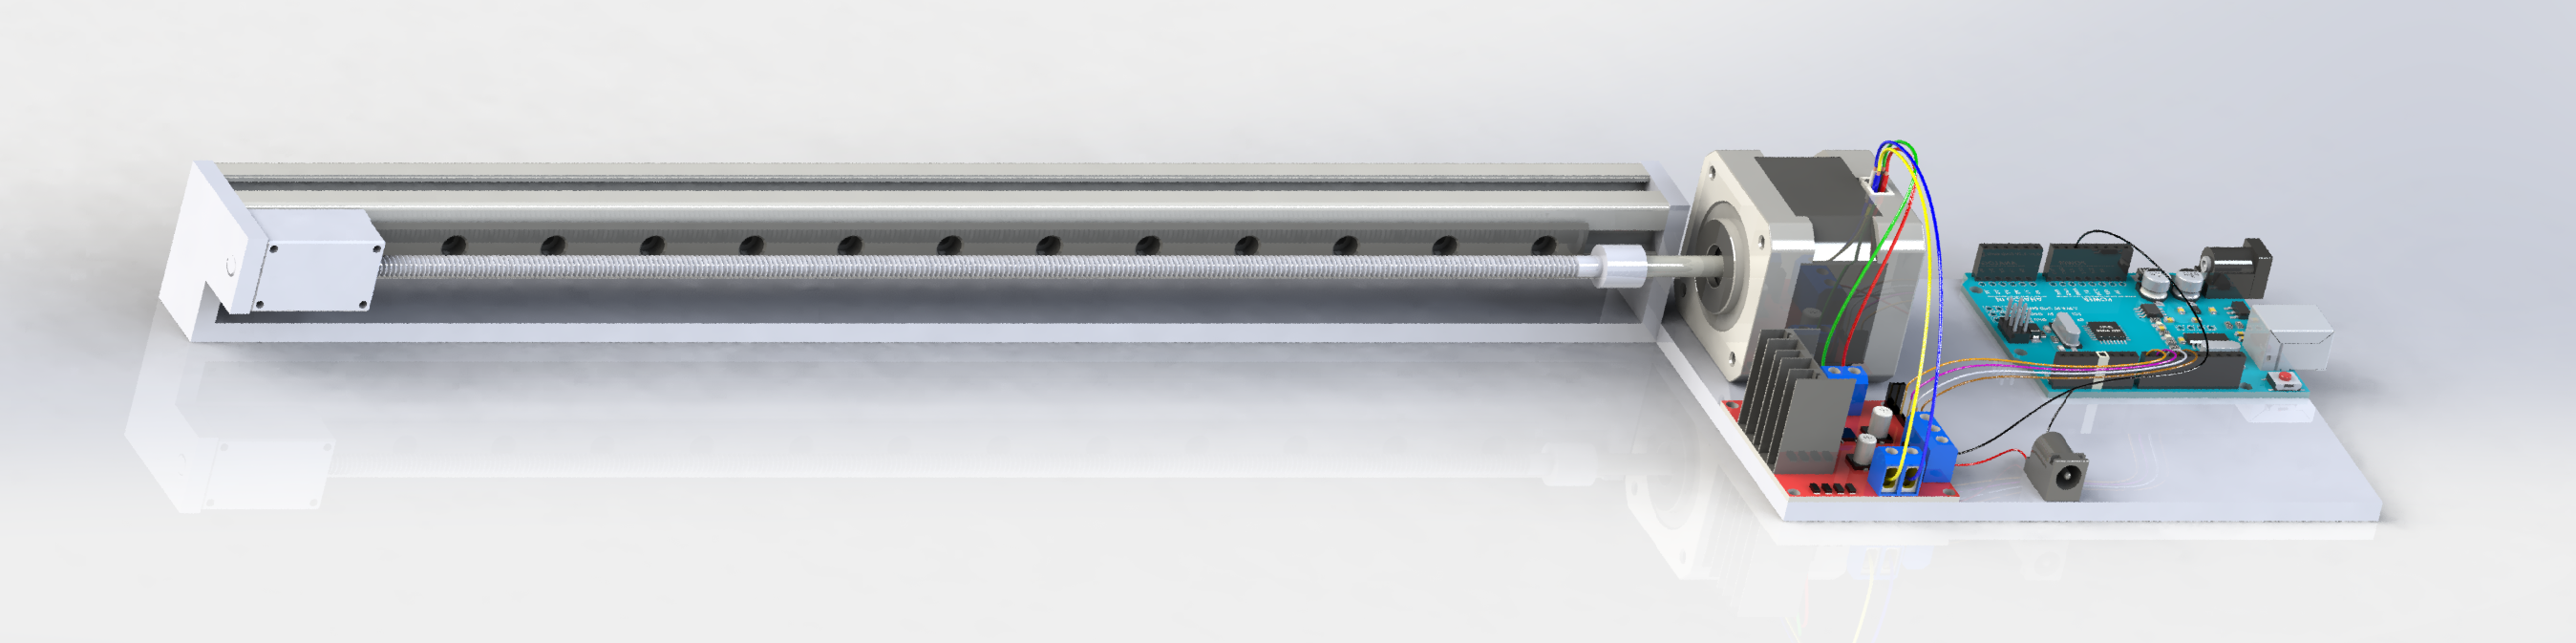
\includegraphics[width=7in]{./images/ASS4-Assembly}}
\caption{General Assembly\label{ASS4-Assembly}}
\end{figure*}

\section{Methodology}

the methodology for this project is organized in three parts, the mechanical system, the electrical system and the software. On each part a introductory discussion about the topic is rendered followed by the necessary explanations relevant to the project. The choices of the project are then explained and justified, including the tools used and relevant data, graph and pictures.
To finalize each part the contributions for the objective is pointed and the section is concluded.


\subsection{Mechanical System}

In factories with or without high levels of automation, linear motion mechanisms are all around. There are many ways to transform rotational motion into linear motion, an well developed mechanism that is used when constant motion or high frequency is required are the Ballscrews. This device provides efficient transmission with low starting torque, smooth running and quite operation. The recirculating ball construction of these type of mechanism results in low friction for smaller drive requirements along with high load capacity. \cite{ref1}

The mechanical system is very similar to the Ballscrew mechanism. It is composed of a base over rail, the rail is designed to restrict the freedom of the base which has four holes to attach any kind of device. The linear movement is achieved by the motor revolutions which is attached to a bolt, when the bolt revolutions cause the base to travel forward and backward inside the rail restriction and through the 305$mm$ allowed for travel. Figure \ref{ASS4-PrinterHead} illustrate the mechanism used in the project.

The rail is mounted onto a bar that is fixed in a metal base and positioned in front of the motor.

This type of linear motion over a screw is used many times in $3D$ printers and other mechanical machinery. 


\begin{figure}[H]
\centerline{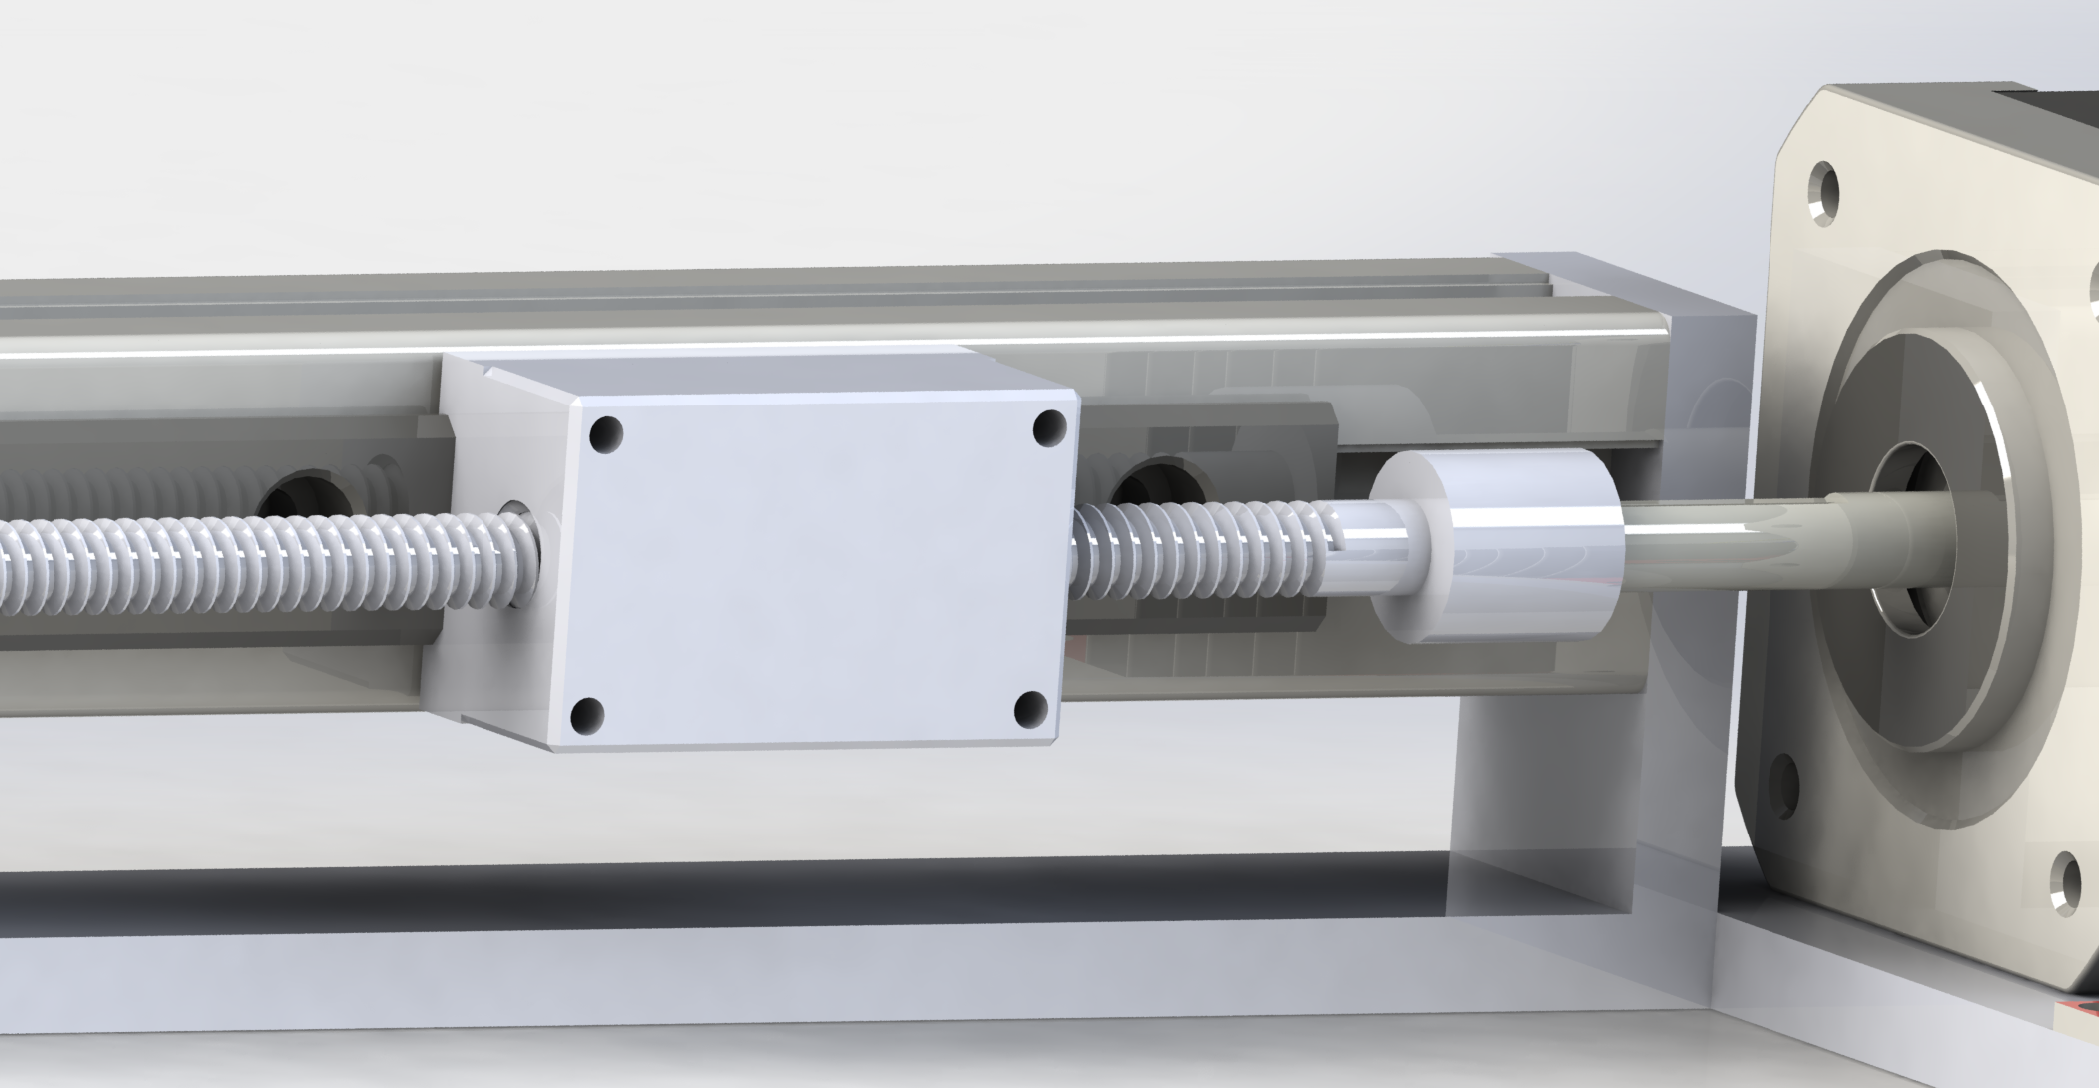
\includegraphics[width=3.5in]{./images/ASS4-PrinterHead}}
\caption{Base over rail\label{ASS4-PrinterHead}}
\end{figure}

To emulate a real interaction between the threads of the base and the linear motion bolt, a $mechanical$ $mate$ was used in Solidworks. With this we can move the base and the linear motion bolt will move accordingly in real time and with the right proportion. Also the threads on the base and on the linear motion bolt were made with standard M12 1.25 with the $thread$ feature in Solidworks, this can be seen on Figure \ref{ASS4-MechanicalMate}. The video submitted with this report shows the complete movement of full travel along the linear motion bolt.

\begin{figure}[H]
\centerline{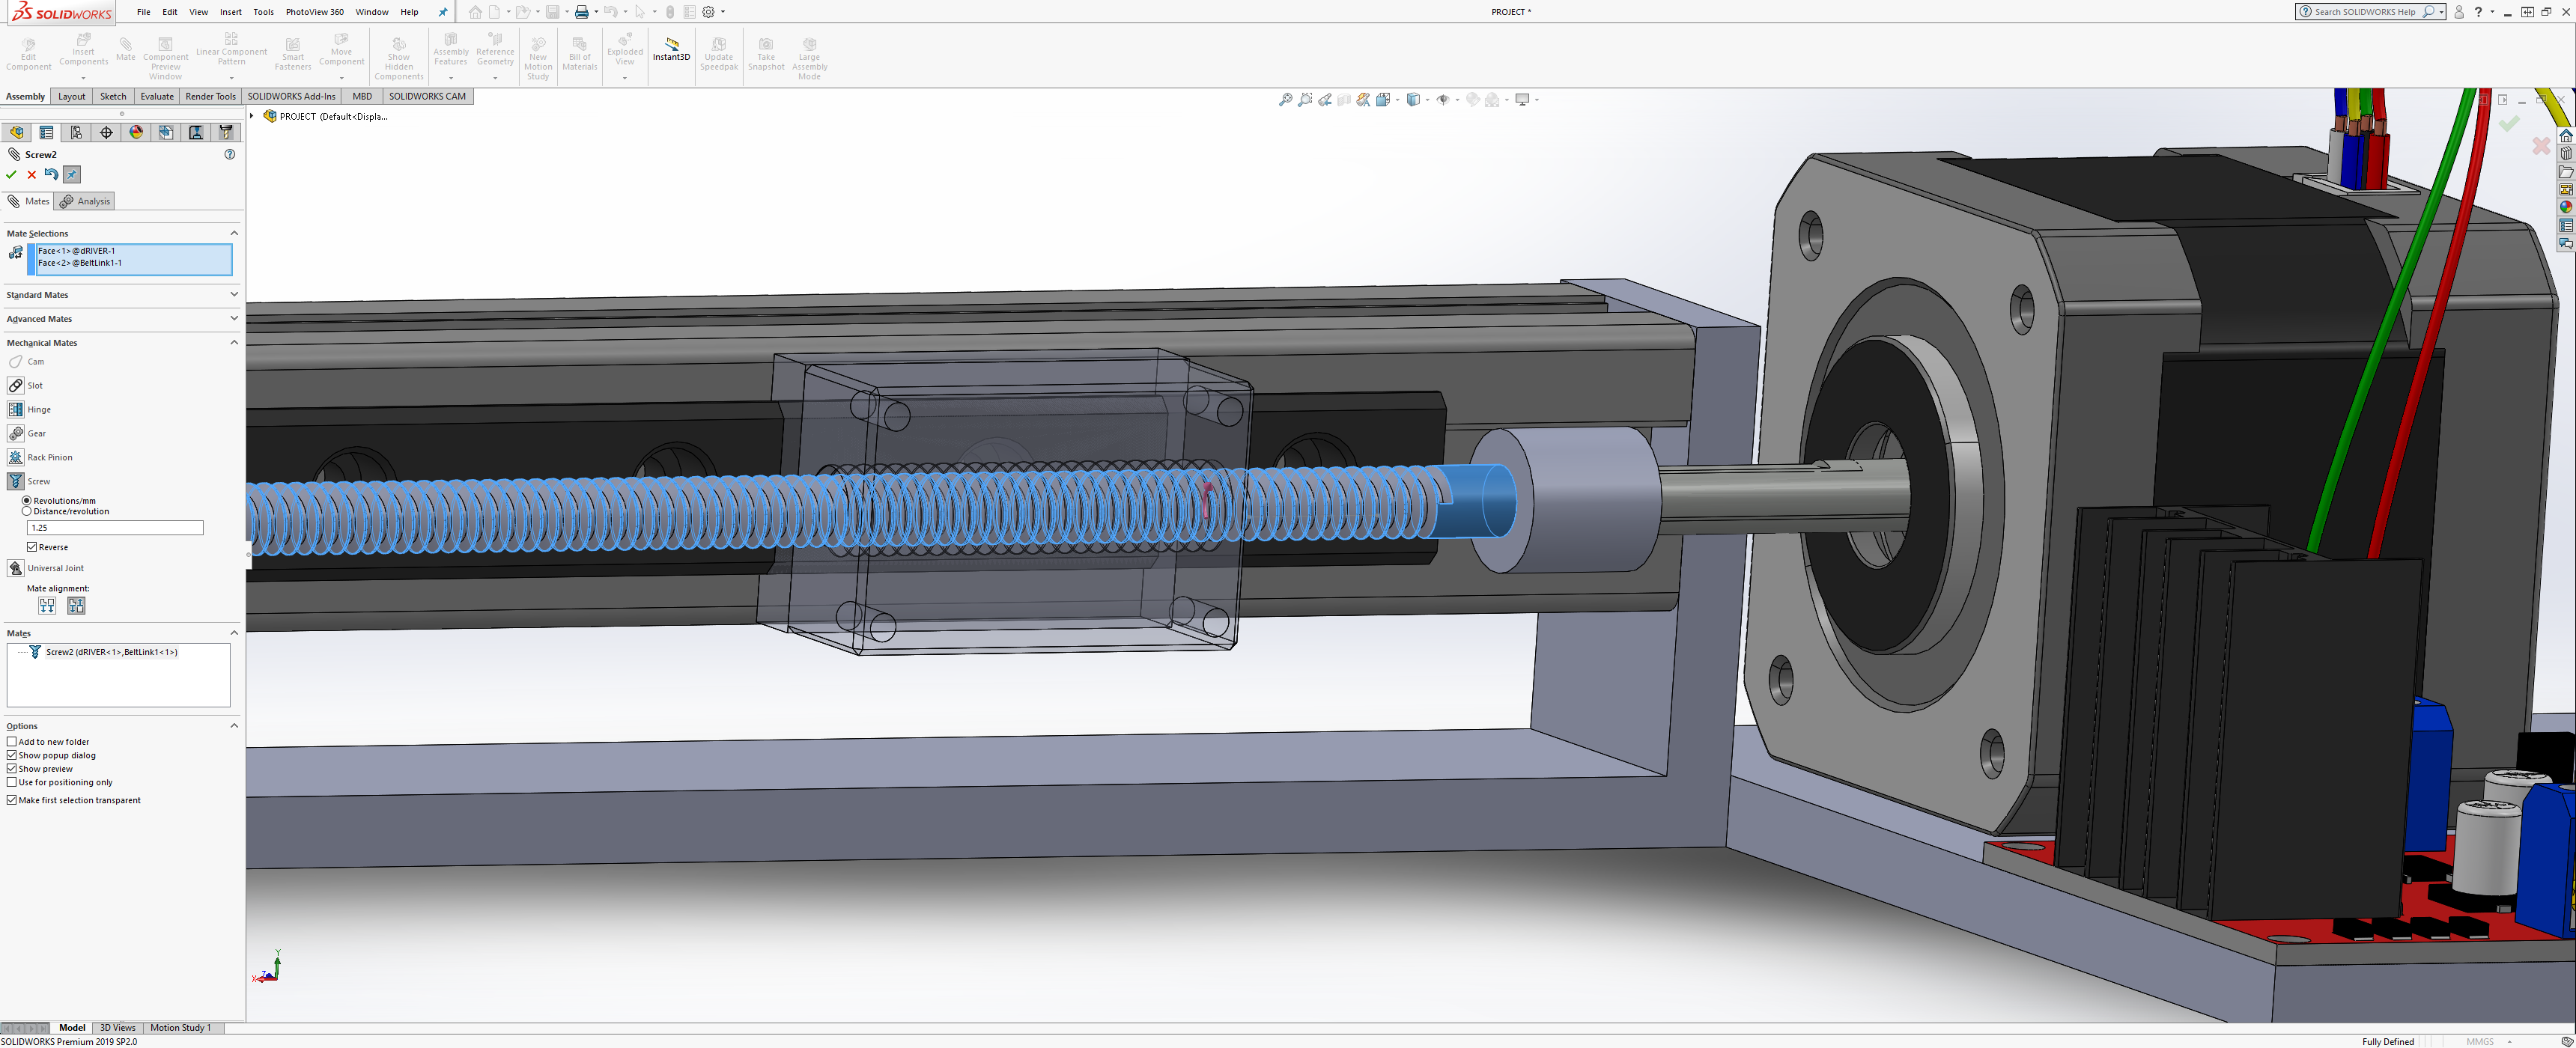
\includegraphics[width=3.5in]{./images/ASS4-MechanicalMate}}
\caption{Mechanical Mate\label{ASS4-MechanicalMate}}
\end{figure}


\subsection{Electrical System}

The electronic system is composed basically by a micro-controller, a H-bridge Motor Driver and a stepper motor. Despite the fact that two power sources is not ideal, there is one power source for the motor and one for the arduino. The motor driver receives ideally 24$V$ and the arduino it's normal  7-12$V$, they share the same ground coming from the arduino ground pin. 


\subsubsection{Motor Driver}


The motor driver is a dual bi-directional one, based on the Dual H-bridge Motor Driver L298. This circuit can control up to 2 motors with 2$A$ each in both directions. It is judge to be ideal for robotics applications and very easy to connect to a micro-controller. \cite{ref2}


\subsubsection{Stepper Motor}

The stepper motor produces rotation through equal angles for each pulse supplied to its input, and these are called steps. Two-phase motors at called bipolar motors and they have four connecting wires for the signal to generate the switching sequence. Figure \ref{ASS4-Stepper} shows the schematics for this kind of motor. \cite{ref3}

\begin{figure}[H]
\centerline{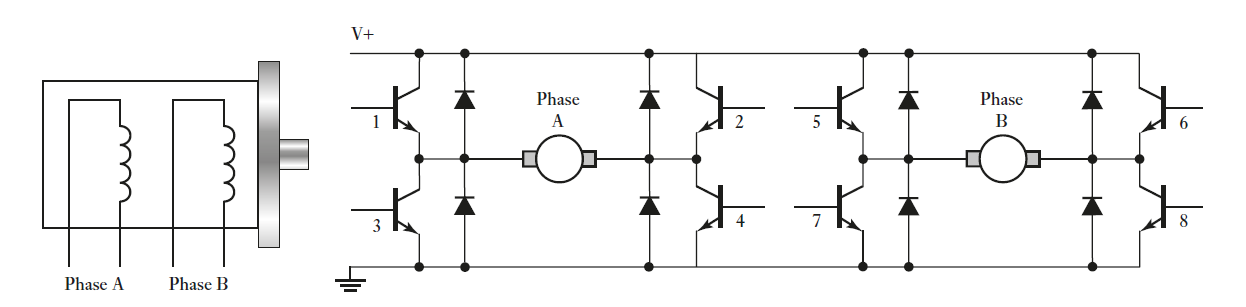
\includegraphics[width=3.5in]{./images/ASS4-Stepper}}
\caption{Stepper motor schematics\label{ASS4-Stepper}}
\end{figure}

The NEMA 17 is a bipolar motor widely used on $3D$ printers, CNC machines and Laser Cutters..\cite{ref5} It is hybrid stepping motor with a 1.8° step angle (200 steps/revolution). Each phase draws 1.2 A at 4 V, allowing for a holding torque of 3.2 kg-cm. It can be operated at lower voltage but torque will drop.

The motor has six wires, connected to two split windings as is common for unipolar stepper motors. Black, Yellow, Green wires is part of first winding where Black is centre tap and Yellow and Green are coil end while Red, White and Blue is part of second winding in which White is centre tap and Red and Blue are coil end wires. Figure \ref{ASS4-Stepper2}, shows the wires colors. \cite{ref7}

\begin{figure}[H]
\centerline{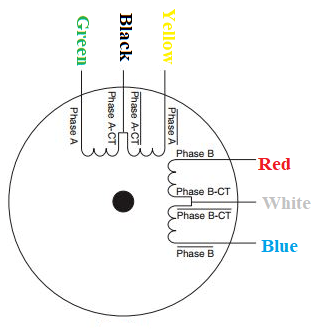
\includegraphics[width=2in]{./images/ASS4-Stepper2}}
\caption{Stepper motor wires\label{ASS4-Stepper2}}
\end{figure}

\subsubsection{Electronic system}

By electronic system in this project we are considering the micro-controller that takes less power then the motor or motor driver. In this case, the motor driver is being driven by an arduino uno, which take 7-12$V$.
The arduino is controlled by the computer via serial port and sends the signal to the motor driver.

\subsubsection{Wiring}

The wires for the model were designed using points located on the path in the parts as can be seem in the Figure \ref{ASS4-Wiring3}. 

\begin{figure}[H]
\centerline{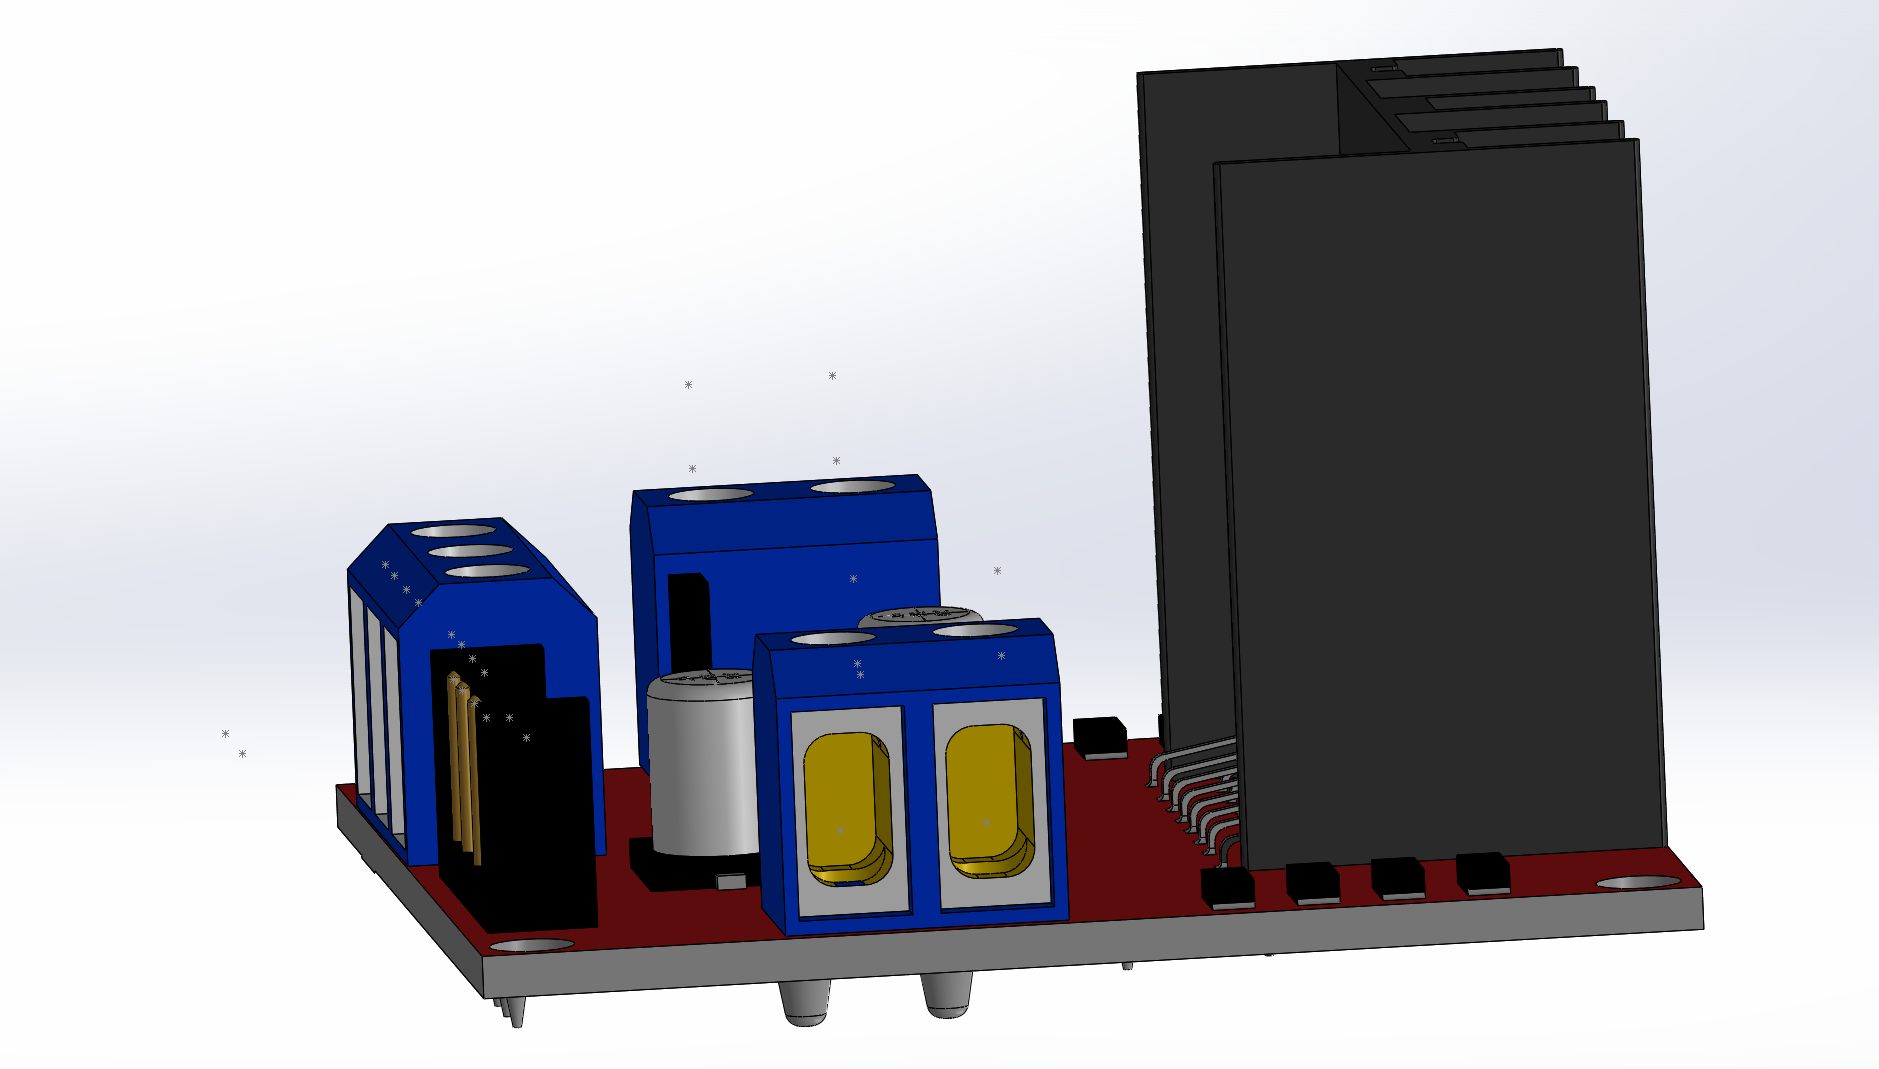
\includegraphics[width=3.5in]{./images/ASS4-Wiring3}}
\caption{Guiding Points\label{ASS4-Wiring3}}
\end{figure}



Then splices could be traced through the desired path simulating this way the behave of real wire, the splices can be seen on Figure \ref{ASS4-Wiring}.


\begin{figure}[H]
\centerline{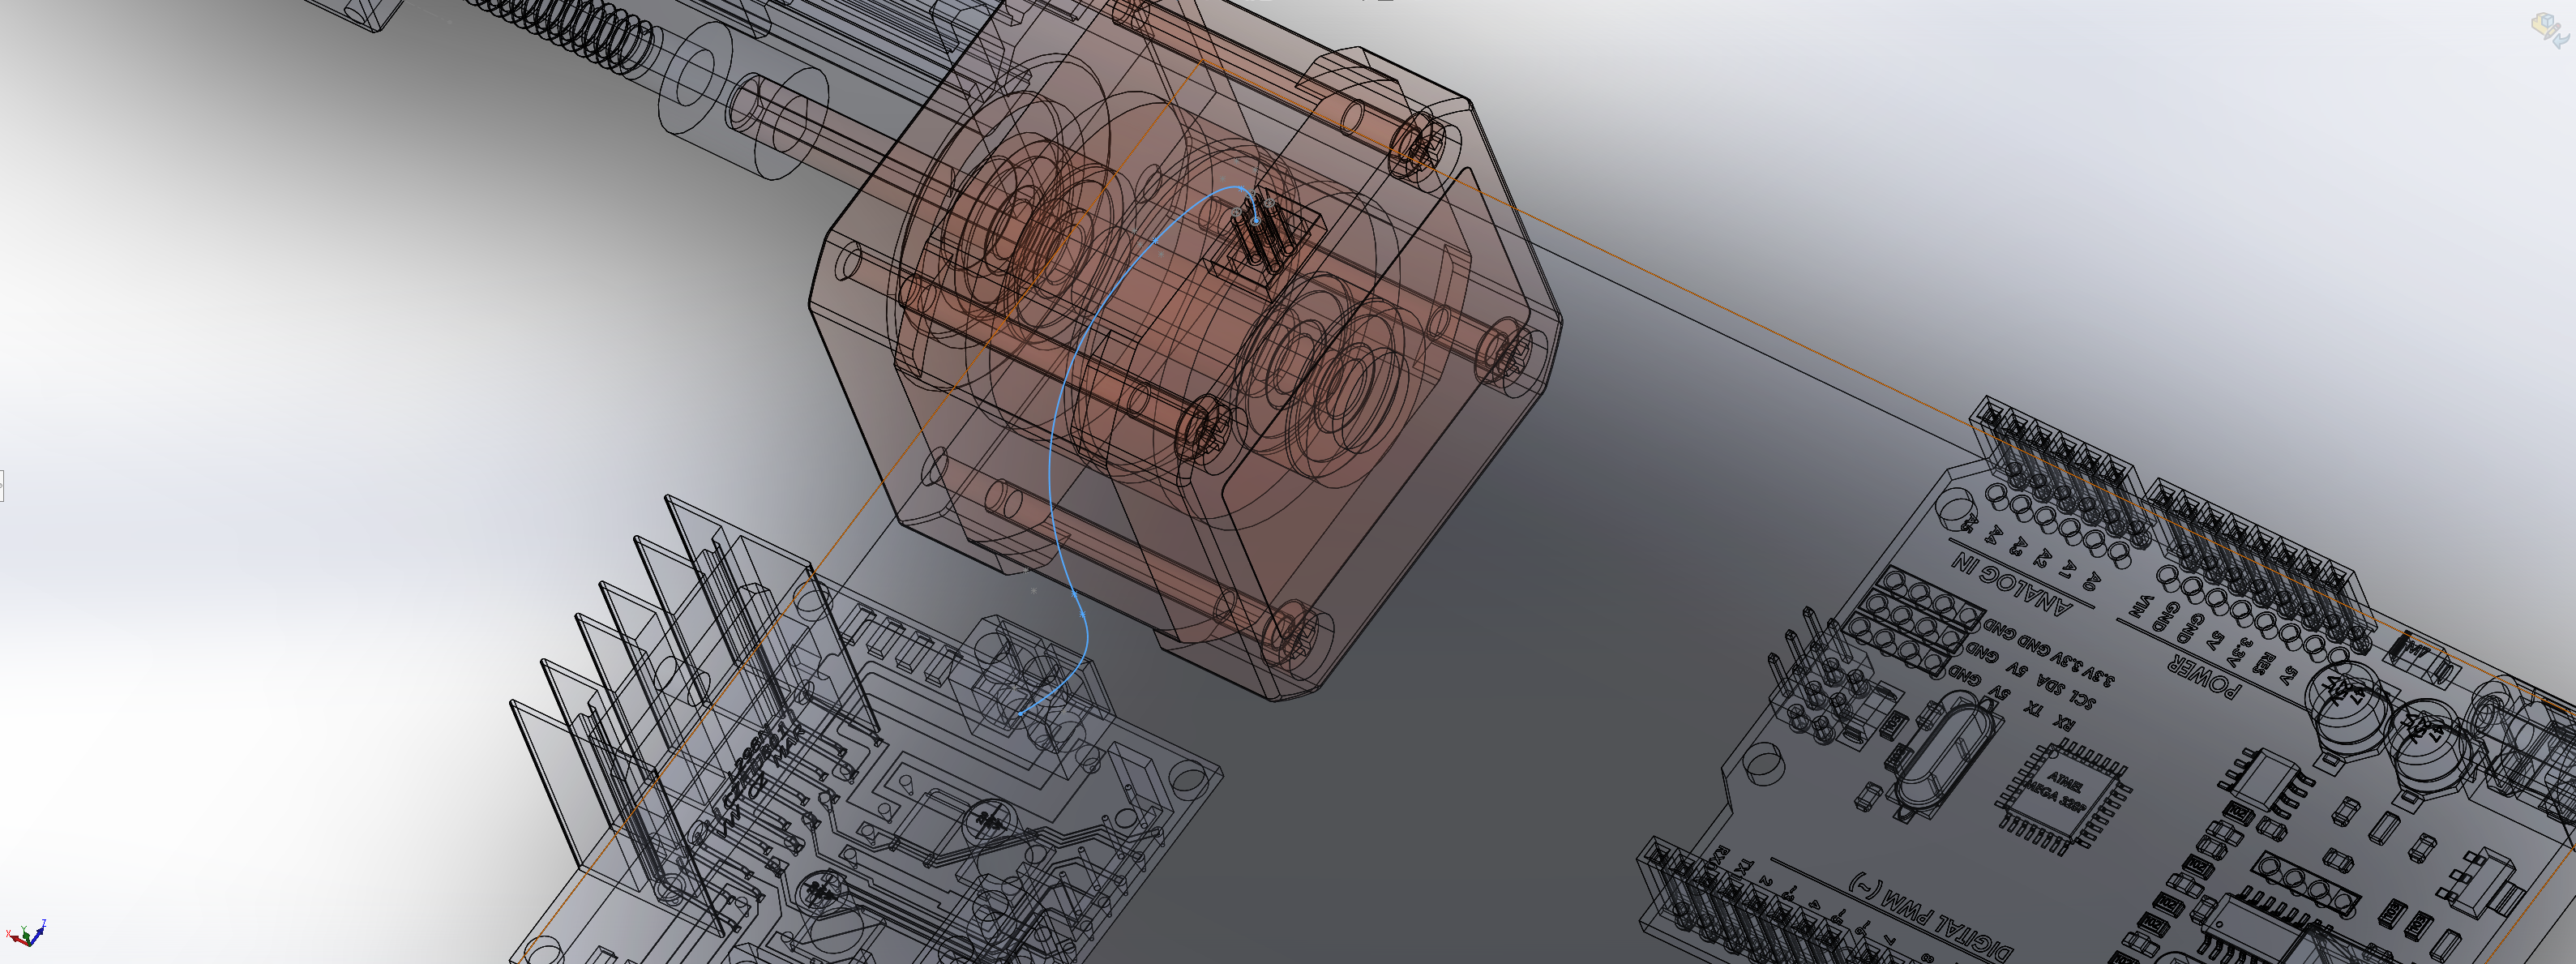
\includegraphics[width=3.5in]{./images/ASS4-Wiring}}
\caption{3D Spline sketch\label{ASS4-Wiring}}
\end{figure}

Figure \ref{ASS4-Wiring4} show the full mounted wires of the motor, motor drive and the arduino.

\begin{figure*}[h]
\centerline{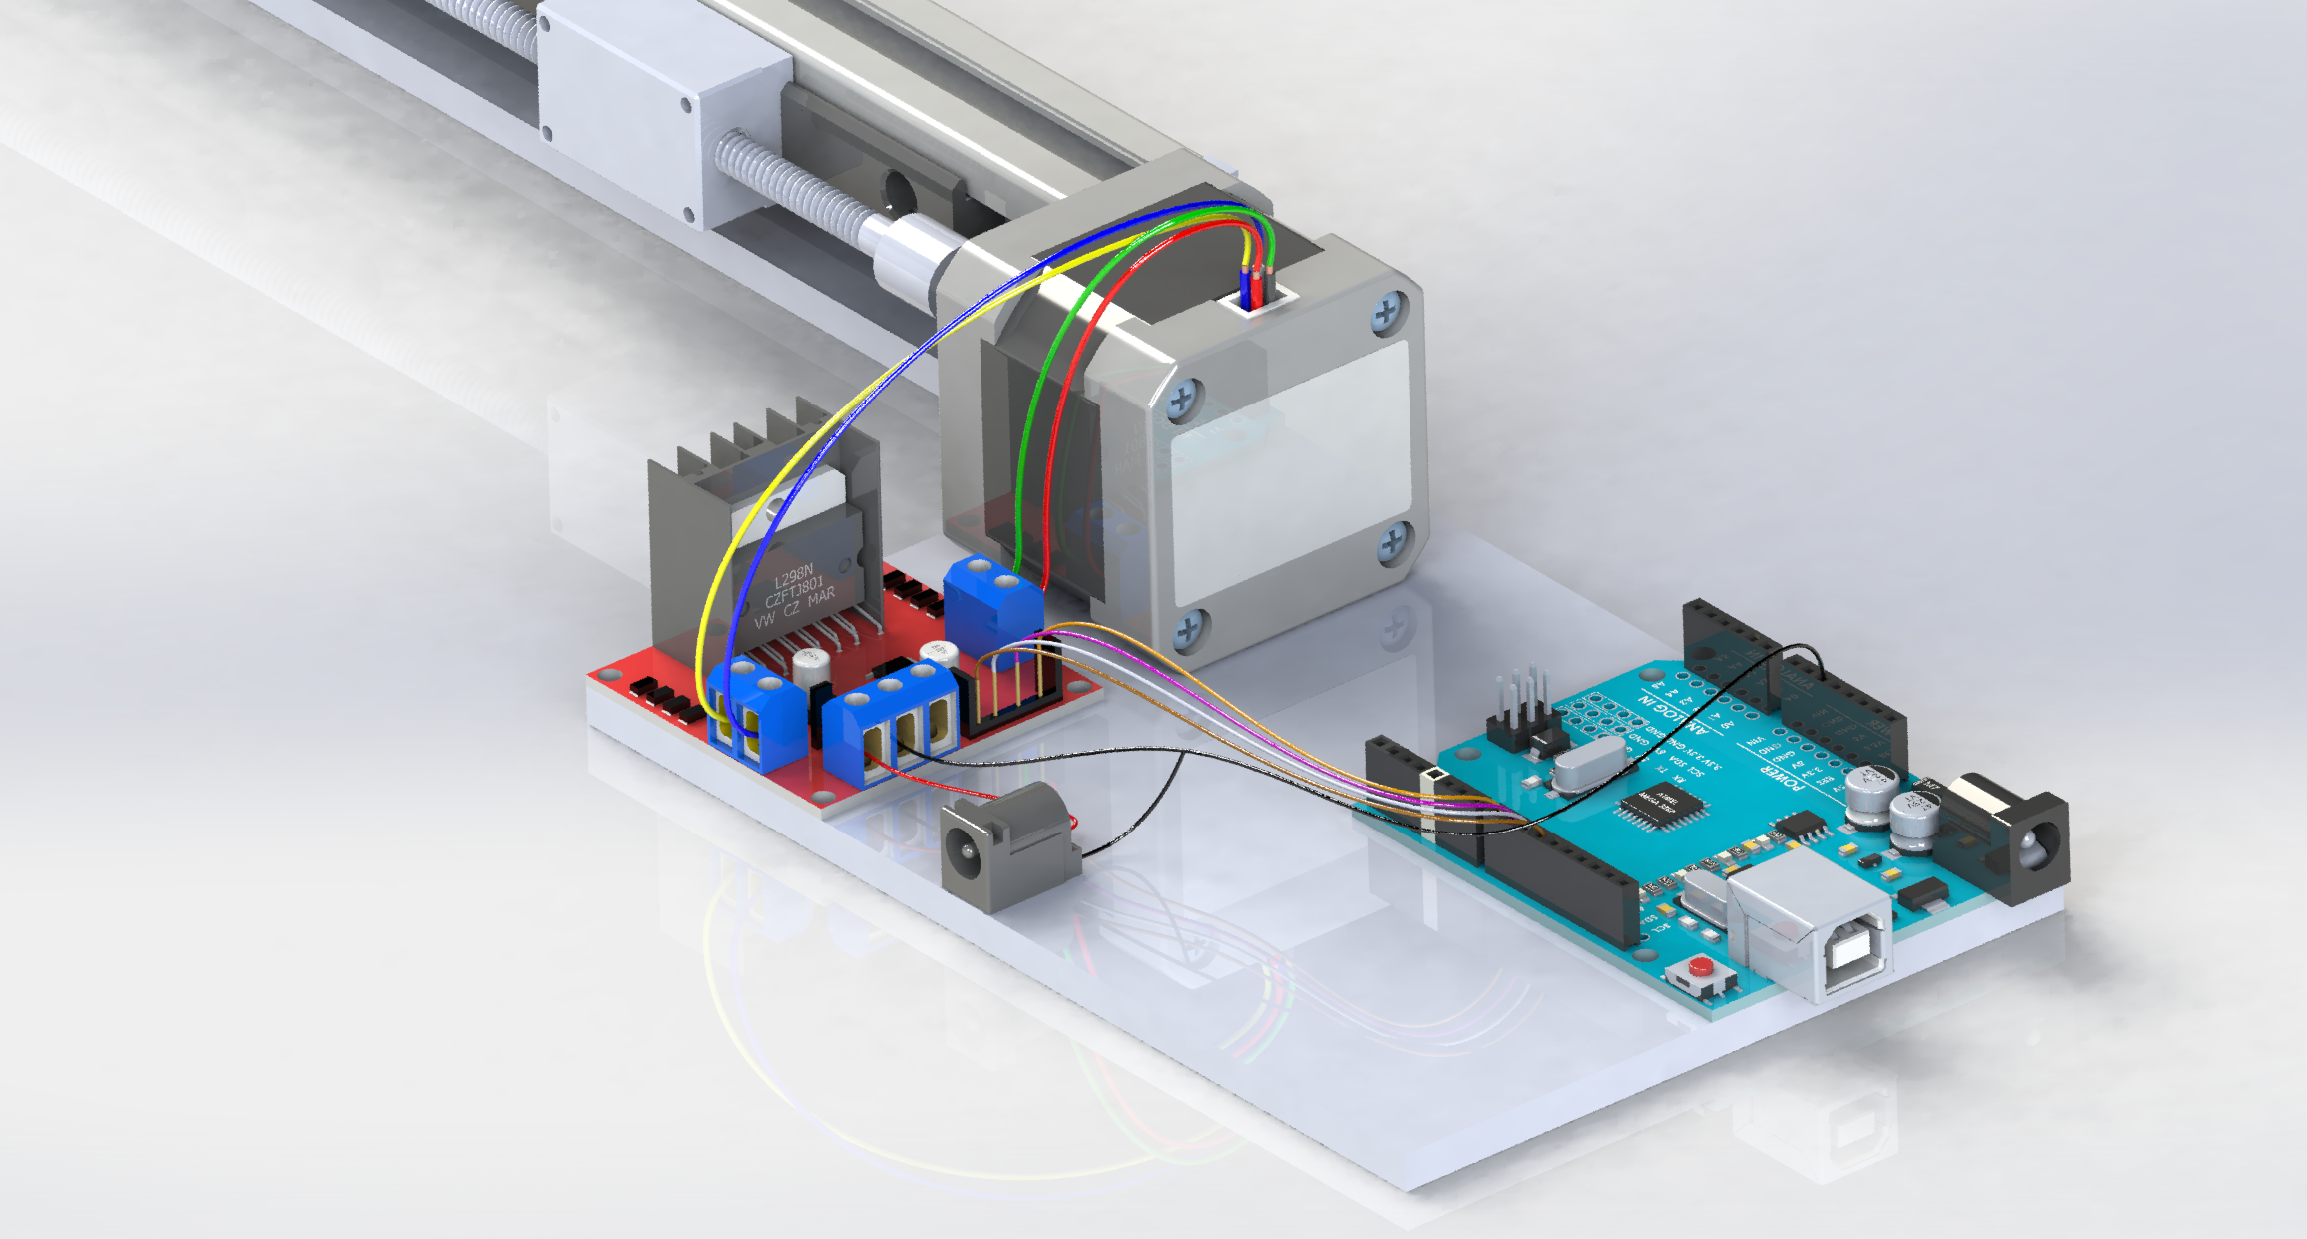
\includegraphics[width=7in]{./images/ASS4-Wiring4}}
\caption{Final Mounted Wires \label{ASS4-Wiring4}}
\end{figure*}


\subsection{Software}
 
The software deployed to this project are written in C++ and developed in two IDE's, being the arduino IDE and Studio Visual Code. Each program make use of external libraries that gives capabilities that the core libraries don't. In the sections below the use of such libraries are 
justified and its works explained.

 
\subsubsection{PC Controls}

The PC control program has five functions that are called accordingly with which option the user chooses from the user interface. The UI is a command line list of options with the five functions and a $Q$ option for quit, Figure \ref{ASS4-VSCode} shows the user interface in action. This functions can be called from a QT button, although this was not implemented its mentioned on the future improvements for the project. The program loops through a $jump()$ function that calls the functions by its number that comes from the $prompt()$ function as can be seeing at the Listing 3 in the appendix. A particular aspect of this structure is the an array of functions is used and the function number will be the number of the element of the array.


\begin{figure*}[h]
\centerline{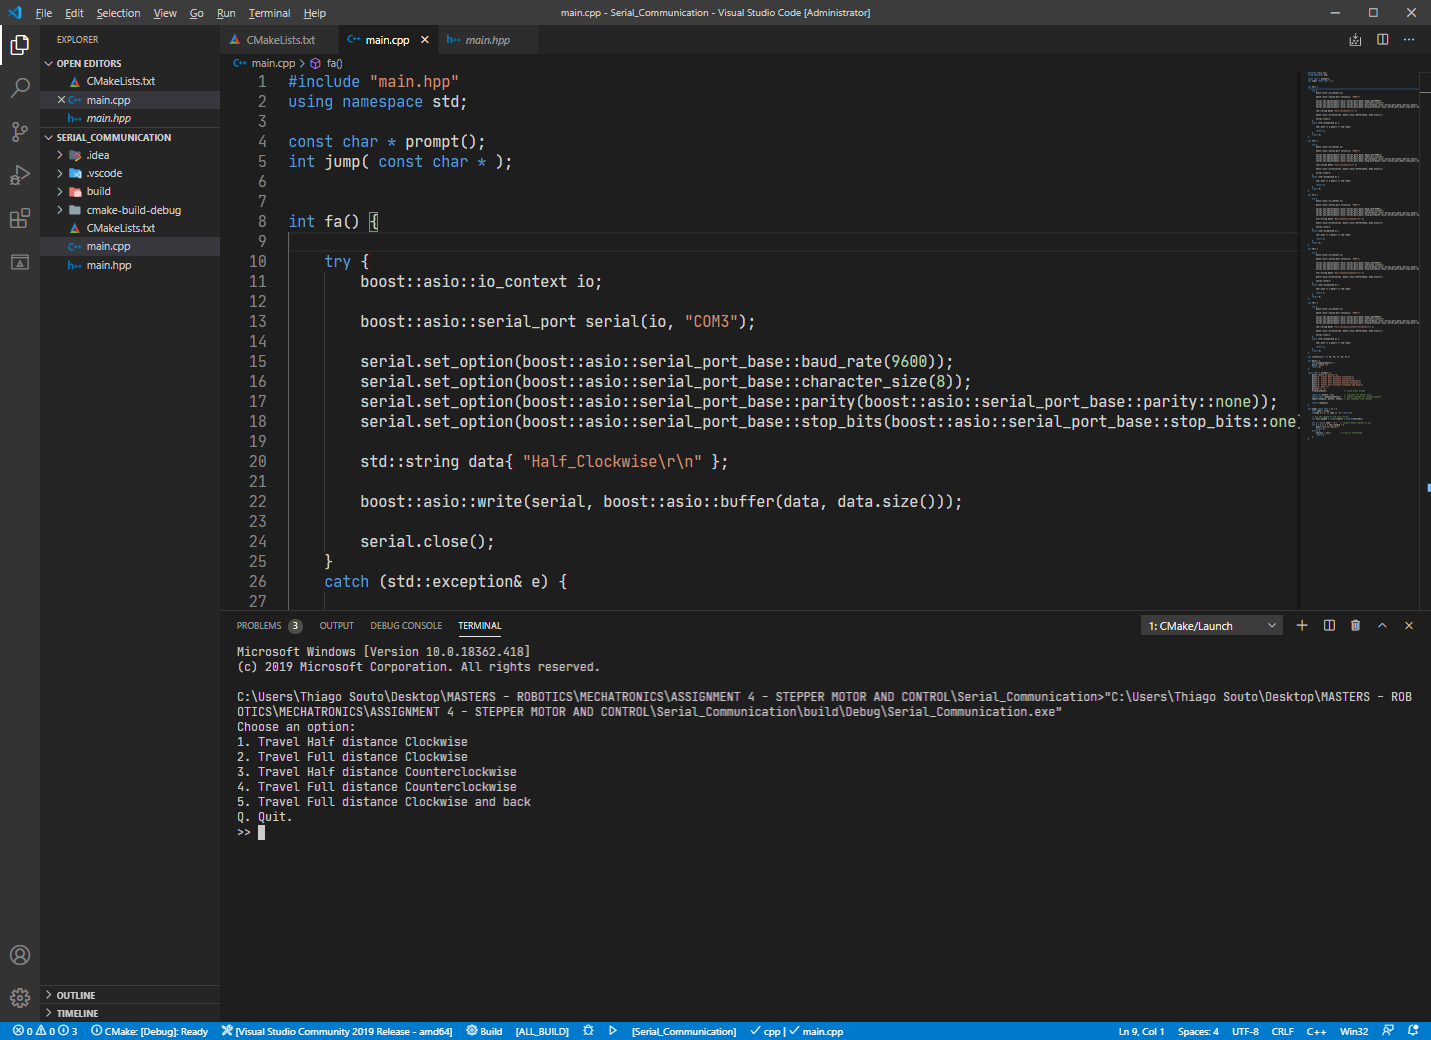
\includegraphics[width=6in]{./images/ASS4-VSCode}}
\caption{Program running at Visual Studio Code \cite{ref2}\label{ASS4-VSCode}}
\end{figure*}

Another aspect of the PC program is the use of the boost library for serial communication. The boost libraries actually emphasize libraries that work well with the C++ Standard Library, it is very useful and used across a wide range of applications. In this case an $asio::io_context$ is created and a serial port assigned to it, the COM3. The options for the serial communication are then set, including $baud rate$, $character_size$, $parity$ and $stop bits$. After that a string is passed through the serial communication and the communication is closed. Any exceptions are treated with an $e.what()$ response printed to the console.


\subsubsection{Micro-controller}


The external library used for the arduino is the stepper motor control library. It sets the steps per revolution varialbe to 200, since the NEMA 17 has a step angle of 1.8$^{\circ}$, and dividing 360$^{\circ}$ by 1.8 give us the 200 steps per revolution set, it also sets a speed of 60 and the serial port baud rate equal to the PC controller so they can communicate and understand each other commands.

It has two functions besides the main loop and the setup, one to receive the messages, which receives every character until the flag character is received and turns the $newData$ variable true and the other function that if $newData$ is true it interpret the message and through the $myStepper.step()$ function rotates the stepper motor accordingly. 

\subsubsection{Control Methodology}

The control methodology consists in a loop that receives the message from the PC and execute the task using the two functions described above. This could be improved by adding a encoder system to know the location  of the head and interpret any position which is commonly made in every application of this motor.


\section{Design Process}


The phases of the project were composed by the ideation and understanding phase, where the problem was studied and some research, mainly in books and the internet, were conducted. Taking into consideration that the research pointed out that the motor was widely used for the purpose of $3D$ printing, CNC, and alike tools, was decided that a base for a printer head that can be transformed into any other tools was a very good case to be exploited.

With the objective in mind and the clear idea of what to design the mechanical model started to get shape by first defining the physical parts of the project and modelling the components that needed to be modelled. With the basic design elaborated some calculations we made possible like the size of the travel and the thread lead, as well as the components attached to the motor and the size of the base.

The third phase of the design consisted in develop the programming necessary to control the system and how to connect the electronic elements of the project. After the definition of the behaviour of the system a mechanical simulation could take place.

To model and simulate the system once more Solidworks was used due to the capabilities that allow the user to combine electrical and mechanical systems as well as animating the model, as can be seen on the video submitted together with this paper. The motion study was a very simple one since the 1 degree-of-freedom system don't allow for much motion.

An interesting aspect of the model was the wiring that allowed to visualize the model in a "real" situation, should it be a more complex model the wires and cables could have been modelled to real size and their organization inside the enclosure or wherever they could be going could easily be studied. 

An advance that could be implemented is to use other software such as Openmodelica or Matlab Simulink to actually build the whole system, these software allow for a complete experience including user experience and real time simulation.

\subsection{Mechanical Simulation}

The mechanical simulation was made using the Solidworks motion studio, the simulation is attached to the submission of this report. In this simulation the base travels the whole distance of the linear motion bolt. In the video the thread of the linear motion bolt as well as the adapter to attach it to the motor axis can be seen in motion.

The $mate$ used to make the animation was a distance make with distance delimitation, the base can could only travel between the range stipulated as can be see at the Figure \ref{ASS4-DistanceMate}, the base can travel from 5$mm$ to 310$mm$ giving a total travel distance of 305$mm$.

\begin{figure}[H]
\centerline{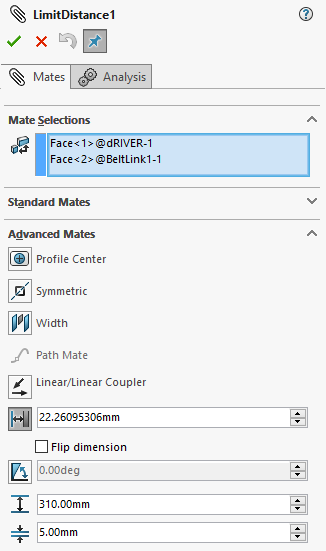
\includegraphics[width=2in]{./images/ASS4-DistanceMate}}
\caption{Distance Mate\label{ASS4-DistanceMate}}
\end{figure}

The amount of revolutions necessary to travel full distance on the screw is equal to the full length of the screw (305 mm) divided by the thread lead (1.25 mm) which is equal to 244 revolutions.



\section{Results}


By taking into consideration the graph shown at Figure \ref{ASS4-RPM-Nema}, which refers to the Torque vs. $rpm$ for the NEMA17 motor we can assume that the motor will maintain a constant torque using 24$V$ until it reaches 300$rpm$. As calculated before, the amount of revolutions necessary to complete the full length travel is 244 revolutions, dividing this by 5$rps$ we find that the full travel will take 48.8$s$ to be completed without decreasing the torque that will be over 40 $N-cm$. \cite{ref5}

If 48$V$ were to be applied the travel time would decrease to 24.4$s$ without loosing torque, but even though, this might not be suitable for some applications and an increased velocity may be implied in, compromising the torque to achieve desired results. Also, the thread lead can be increased so that the amount travelled by revolution would increase, since they are directly proportional.

A maximum of 1800$rpm$, or 30$rps$, would allow the travel time to be decreased to 8.13$s$, although to work on the edge of any system is not recommended 


Currently Desktop $3D$ printers can vary the printer head velocity from 40-150$mm/s$, some are even faster then 150$mm/s$, although the quality decreases noticeably after such speeds and the filament tends to slip at these speeds as well. \cite{ref6}

In the current configuration without changing the thread the speed of the system would be between 6.25$mm/s$ to 37.5$mm/s$. Results ranging from ideal to maximum speed and power supply. 


\begin{figure}[H]
\centerline{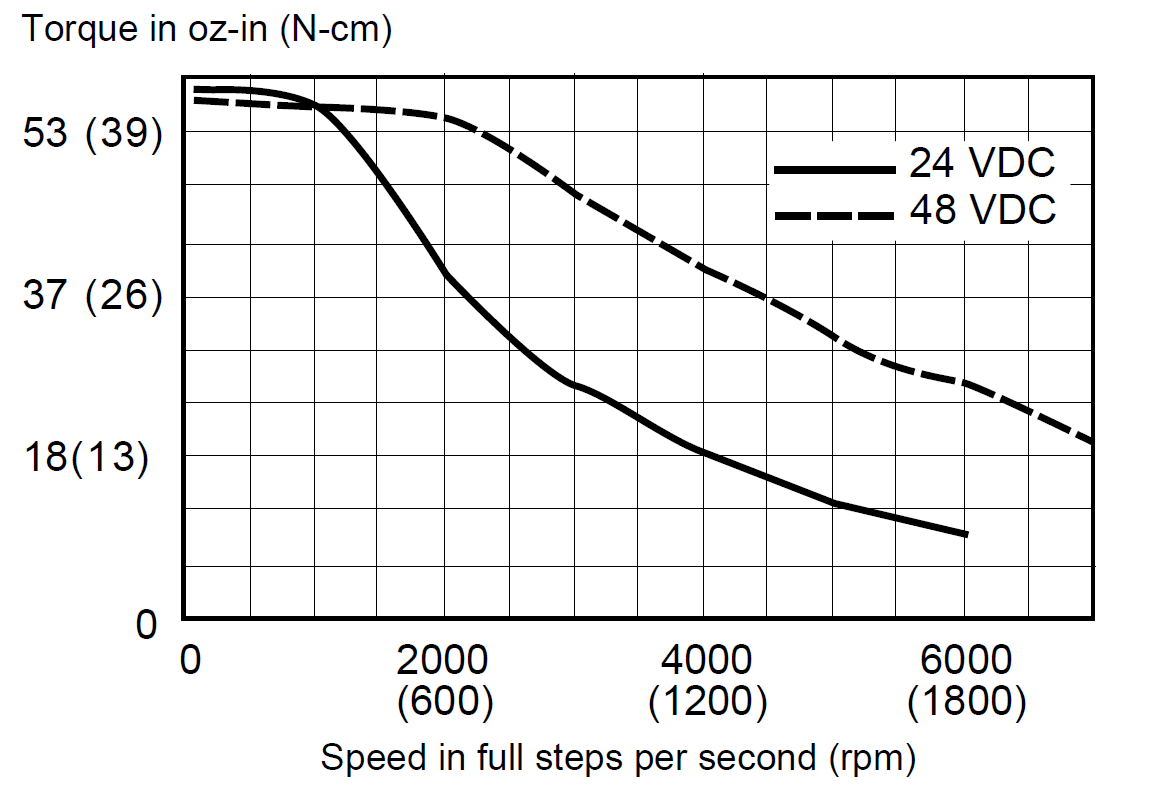
\includegraphics[width=3.5in]{./images/ASS4-RPM-Nema}}
\caption{Torque vs. $rpm$ - NEMA17 \cite{ref5}\label{ASS4-RPM-Nema}}
\end{figure}

\section{Discussion and Conclusions}

In this project two different programs were connected and together with the mechanical and electrical systems were capable to achieve the main objective of the assignment for sure which is to practice the construction of mechatronic systems and integrate them in a useful application.
New knowledge around wire routing in Solidworks, PC based program to control micro-controllers, as well as the functioning of a stepper motor were knowledge outcomes resulted from this report.

The system performance was clear and acceptable, the results were in conformance with the aim of the project, although in need of some adjustments to go beyond the project aim.  

Improvements and recommendations for the project in future developments include the following:


\begin{enumerate}
\item First improvement in this project is clearly to change the thread lead to a degree where a suitable velocity of 100$mm/s$ is achieved. Or to achieve the purpose of the project to which it would be applied, since this factor has the most direct effect on the velocity and that in the project a very narrow gap was used.
\item Design the PC control to send all the measurements necessary to implement a real $3D$ printer is the second improvement, the localization of the printer head can be easily defined by its relation with the thread. 
\item Implement two more motors with respective printer heads and construct a real $3D$ printer is a very good opportunity.
\item To implement other systems, different from the $3D$ printer initiative like transporters of food in a Japanese restaurant, or even a lathe or some other solutions would be the ultimate improvement for this project.
\item Develop a QT user interface for the PC control program.
\end{enumerate}






\clearpage
\newpage

\begin{thebibliography}{00}


\bibitem{ref1} (HIWINF - Linear Motion Products \& Technology - Ballscrews)(2020, June). Linear Motion - New Zealand. Available: http://www.drivehq.com/file/df.aspx/publish/linearmotion/Ballscrews/Ballscrews-Indexed.pdf. 

\bibitem{ref2} (L298N Motor Driver - Datasheet)(2020, June). Available:  http://www.handsontec.com/dataspecs/L298N\%20Motor\%20Driver.pdf.

\bibitem{ref3} W. Bolton, \emph{Mechatronics - Electronic control systems in mechanical and electrical engineering}. United Kingdom: Pearson Education Limited, 2019.

\bibitem{ref4} (16x2 LCD Module) Datasheet. (2020, May).  Available: https://components101.com/16x2-lcd-pinout-datasheet.


\bibitem{ref5} (NEMA17 stepper motor Quick Reference R060210)(2020, June). Schneider Electric Motion USA. Available: https://datasheetspdf.com/pdf-file/1260602/Schneider/NEMA17/1. 

\bibitem{ref6} (All3dp website)(2020, June). Available: https://all3dp.com/3d-printing-speed/:~:text=Currently\%2C\%20there\%20are\%20generally\%20three,faster\%20than\%20150\%20mm\%2Fs.s.

\bibitem{ref7} (101 Components - NEMA 17)(2020, June). Available: https://components101.com/motors/nema17-stepper-motor.



\end{thebibliography}

\clearpage
\newpage

\onecolumn

\appendix


\begin{lstlisting}[language=C++, caption=PC controller program - Serial Communication - Header file]
#ifndef SERIAL_COMMUNICATION_MAIN_H
#define SERIAL_COMMUNICATION_MAIN_H

#include <iostream>
#include <boost/asio.hpp>
#include <cstdio>

#endif //SERIAL_COMMUNICATION_MAIN_H
\end{lstlisting}

\begin{lstlisting}[language=C++, caption=PC controller program - Serial Communication - CMake file]
cmake_minimum_required(VERSION 3.16)
project(Serial_Communication)

set(CMAKE_CXX_STANDARD 17)

set(CMAKE_INCLUDE_CURRENT_DIR ON)

find_package(Boost)

if (NOT boost_FOUND)

    set(Boost_INCLUDE_DIR "C:/boost")
    set(Boost_LIBRARY_DIRS "C:/boost/stage/lib")
    set(Boost_LIBRARIES "")

endif()

include_directories(${Boost_INCLUDE_DIR})
link_directories(${Boost_LIBRARY_DIRS})

add_executable(Serial_Communication main.cpp main.hpp)
target_link_libraries(Serial_Communication ${Boost_LIBRARIES})

# Utilities

set(CMAKE_DIR "C:/Cmake")
find_program(CMAKE_EXECUTABLE NAMES cmake HINTS ${cmake_dir} ENV CMAKE_DIR PATH_SUFFIXES bin)

# Build

set_property(TARGET Serial_Communication PROPERTY CXX_STANDARD 17)

# Install

install(TARGETS Serial_Communication DESTINATION ${PROJECT_SOURCE_DIR}/bin)
\end{lstlisting}

\clearpage
\newpage

\begin{lstlisting}[language=C++, caption=PC controller program - Serial Communication - Main file]
#include "main.hpp"
using namespace std;

const char * prompt();
int jump( const char * );


int fa() {

    try {
        boost::asio::io_context io;

        boost::asio::serial_port serial(io, "COM3");

        serial.set_option(boost::asio::serial_port_base::baud_rate(9600));
        serial.set_option(boost::asio::serial_port_base::character_size(8));
        serial.set_option(boost::asio::serial_port_base::parity(boost::asio::serial_port_base::parity::none));
        serial.set_option(boost::asio::serial_port_base::stop_bits(boost::asio::serial_port_base::stop_bits::one));

        std::string data{ "Half_Clockwise\r\n" };

        boost::asio::write(serial, boost::asio::buffer(data, data.size()));

        serial.close();
    }
    catch (std::exception& e) {

        std::cout << e.what() << std::endl;

        return 1;
    }
    return 0;
}

int fb() {

    try {
        boost::asio::io_context io;

        boost::asio::serial_port serial(io, "COM3");

        serial.set_option(boost::asio::serial_port_base::baud_rate(9600));
        serial.set_option(boost::asio::serial_port_base::character_size(8));
        serial.set_option(boost::asio::serial_port_base::parity(boost::asio::serial_port_base::parity::none));
        serial.set_option(boost::asio::serial_port_base::stop_bits(boost::asio::serial_port_base::stop_bits::one));

        std::string data{ "Full_Clockwise\r\n" };

        boost::asio::write(serial, boost::asio::buffer(data, data.size()));

        serial.close();
    }
    catch (std::exception& e) {

        std::cout << e.what() << std::endl;

        return 1;
    }
    return 0;
}

int fc() {

    try {
        boost::asio::io_context io;

        boost::asio::serial_port serial(io, "COM3");

        serial.set_option(boost::asio::serial_port_base::baud_rate(9600));
        serial.set_option(boost::asio::serial_port_base::character_size(8));
        serial.set_option(boost::asio::serial_port_base::parity(boost::asio::serial_port_base::parity::none));
        serial.set_option(boost::asio::serial_port_base::stop_bits(boost::asio::serial_port_base::stop_bits::one));

        std::string data{ "Half_Counterclockwise\r\n" };

        boost::asio::write(serial, boost::asio::buffer(data, data.size()));

        serial.close();
    }
    catch (std::exception& e) {

        std::cout << e.what() << std::endl;

        return 1;
    }
    return 0;
}

int fd() {

    try {
        boost::asio::io_context io;

        boost::asio::serial_port serial(io, "COM3");

        serial.set_option(boost::asio::serial_port_base::baud_rate(9600));
        serial.set_option(boost::asio::serial_port_base::character_size(8));
        serial.set_option(boost::asio::serial_port_base::parity(boost::asio::serial_port_base::parity::none));
        serial.set_option(boost::asio::serial_port_base::stop_bits(boost::asio::serial_port_base::stop_bits::one));

        std::string data{ "Full_Counterclockwise\r\n" };

        boost::asio::write(serial, boost::asio::buffer(data, data.size()));

        serial.close();
    }
    catch (std::exception& e) {

        std::cout << e.what() << std::endl;

        return 1;
    }
    return 0;
}

int fe() {

    try {
        boost::asio::io_context io;

        boost::asio::serial_port serial(io, "COM3");

        serial.set_option(boost::asio::serial_port_base::baud_rate(9600));
        serial.set_option(boost::asio::serial_port_base::character_size(8));
        serial.set_option(boost::asio::serial_port_base::parity(boost::asio::serial_port_base::parity::none));
        serial.set_option(boost::asio::serial_port_base::stop_bits(boost::asio::serial_port_base::stop_bits::one));

        std::string data{ "Full_Clockwise_Counterclockwise\r\n" };

        boost::asio::write(serial, boost::asio::buffer(data, data.size()));

        serial.close();
    }
    catch (std::exception& e) {

        std::cout << e.what() << std::endl;

        return 1;
    }
    return 0;
}

int (*funcs[])() = { fa, fb, fc, fd, fe };

int main() {
    while(jump(prompt())) ;
    puts("\nDone.");
    return 0;
}

const char * prompt() {
    puts("Choose an option:");
    puts("1. Travel Half distance Clockwise");
    puts("2. Travel Full distance Clockwise");
    puts("3. Travel Half distance Counterclockwise");
    puts("4. Travel Full distance Counterclockwise");
    puts("5. Travel Full distance Clockwise and back");
    puts("Q. Quit.");
    printf(">> ");
    fflush(stdout);                 // flush after prompt
    
    const int buffsz = 16;          // constant for buffer size
    static char response[buffsz];   // static storage for response buffer
    fgets(response, buffsz, stdin); // get response from console
    
    return response;
}

int jump( const char * rs ) {
    char code = rs[0];
    if(code == 'q' || code == 'Q') return 0;
    
    // get the length of the funcs array
    int func_length = sizeof(funcs) / sizeof(funcs[0]);
    
    int i = (int) code - '0';   // convert ASCII numeral to int
    if( i < 1 || i > func_length ) {
        puts("invalid choice");
        return 1;
    } else {
        funcs[i - 1]();         // array is zero-based
        return 1;
    } 
}
\end{lstlisting}


\clearpage
\newpage

\begin{lstlisting}[language=C++, caption=Micro-controller - Motor Control]
// Include the Arduino Stepper Library
#include <Stepper.h>

// Number of steps per output rotation
const int stepsPerRevolution = 200;

// Create Instance of Stepper library
Stepper myStepper(stepsPerRevolution, 8, 9, 10, 11);

const byte numChars = 32;
char receivedChars[numChars];

boolean newData = false;


void setup(){
    // set the speed at 60 rpm:
    myStepper.setSpeed(60);
    // initialize the serial port:
    Serial.begin(9600);
}

void loop(){
    recvWithEndMarker();
    controlMotor();
}


void recvWithEndMarker(){
    static byte ndx = 0;
    char endMarker = '\n';
    char rc;

    while(Serial.available() > 0 && newData == false){
        rc = Serial.read();

        if(rc != endMarker){
            receivedChars[ndx] = rc;
            ndx++;
            if(ndx >= numChars){
                ndx = numChars -1;
            }
        }
        else{
            receivedChars[ndx] = '\0'; // Terminate the string
            ndx = 0;
            newData = true;
        }
    }   
}


void controlMotor(){
    if (newData == true && receivedChars == "Half_Clockwise") {
        // step five revolutions in one direction:
        myStepper.step(122*stepsPerRevolution);
    } else if (newData == true && receivedChars == "Full_Clockwise") {
        // step ten revolutions in one direction:
        myStepper.step(244*stepsPerRevolution);
    } else if (newData == true && receivedChars == "Half_Counterclockwise") {
        // step ten revolutions in one direction:
        myStepper.step(-122*stepsPerRevolution);
    } else if (newData == true && receivedChars == "Full_Counterclockwise") {
        // step ten revolutions in one direction:
        myStepper.step(-244*stepsPerRevolution);
    } else if (newData == true && receivedChars == "Full_Clockwise_Counterclockwise") {
        // step ten revolutions in one direction:
        myStepper.step(244*stepsPerRevolution);
        delay(500);
        // step ten revolutions in the other direction:
        myStepper.step(-244*stepsPerRevolution);
    }    
    delay(500);          
    newData = false;
}

\end{lstlisting}

\end{document}
